\documentclass[11pt]{article}
\usepackage[utf8]{inputenc}
\usepackage[top=60pt, bottom=60pt, left=70pt, right=70pt]{geometry}
\usepackage{graphicx}
% Default fixed font does not support bold face
\DeclareFixedFont{\ttb}{T1}{txtt}{bx}{n}{8} % for bold
\DeclareFixedFont{\ttm}{T1}{txtt}{m}{n}{8}  % for normal

% Custom colors
\usepackage{color}
\definecolor{deepblue}{rgb}{0,0,0.5}
\definecolor{deepred}{rgb}{0.6,0,0}
\definecolor{deepgreen}{rgb}{0,0.5,0}
\definecolor{commentgrey}{rgb}{0.5,0.5,0.5}
\usepackage{listings}

% Python style for highlighting
\lstset{
language=Python,
basicstyle=\ttm,
otherkeywords={self},             % Add keywords here
keywordstyle=\ttb\color{deepblue},
emph={MyClass,__init__},          % Custom highlighting
emphstyle=\ttb\color{deepred},    % Custom highlighting style
stringstyle=\color{deepgreen},
frame=tb,                         % Any extra options here
commentstyle=\color{commentsgrey}
}


\title{Examples}
\author{Daniel W. Zaide}

\begin{document}

\maketitle
\section{A simple nonlinear set of equations}
This example is implemented in {\bf example.py}. All implementation details are in that file. Only the math is shown here. Consider the two block system, with three equations,
\begin{eqnarray*}
C_f(u_1 - u_0) + C_su_1 = 0 \\ C_f(u_2 - u_1) + C_su_2 = 0 \\ (v_1-u_2) - g(v_1)v_1 = 0
\end{eqnarray*}
For some constants $C_f, C_s$ and some function $g(v_1)$. The unknowns are $u_1,u_2$, and $v_1$, with a boundary block containing $u_0$. There are two flux functions, one for U and one for V
\[
F_u(U,U_N) = C_f(U-U_N), \qquad F_v(V,U_N) = V-U
\]

and two source functions,
\[
S_u(U) = C_sU, \qquad S_v(U) = -g(U)U
\]
illustrated in Figure \ref{fig:ex1}.
\begin{figure}[!ht]
\centering
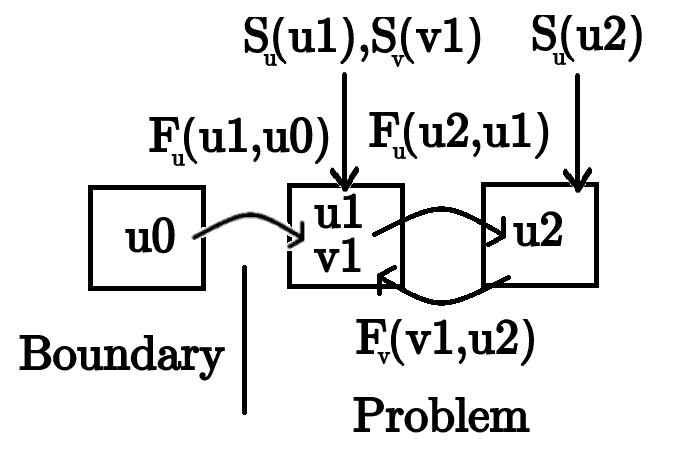
\includegraphics[width=0.3\textwidth]{images/example1.png}
\caption{A simple nonlinear example with boundary conditions.}
\label{fig:ex1}
\end{figure}


If we choose $u_0 = C_s = C_f = 1$ and $g(U) = U$, the system has one unique solution,
\[
u_1 = \frac{1}{2}, \qquad u_2 = \frac{1}{4}, \qquad v_1 = \frac{1}{2}
\]


\subsection{An alternate version}
We could also do away with boundary blocks, and write this using the boundary condition as a source as in Figure \ref{fig:ex2}. The boundary condition is written as a source, with
\[
S_0(U) = C_f(U-U_0)
\]
\begin{figure}[!ht]
\centering
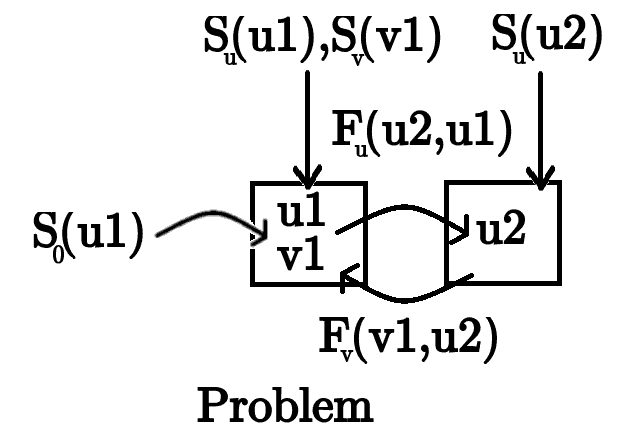
\includegraphics[width=0.3\textwidth]{images/example1a.png}
\caption{A simple nonlinear example with a source as the boundary condition.}
\label{fig:ex2}
\end{figure}
Both versions are valid and equivalent, and will depend on how the system is framed.

\section{Poisson's Equation}
This is solved in the file {\bf poisson2D.py} and all implementation details are in the function. Only the math is shown here. Consider the decoupled pair of Poisson's equations, $\nabla^2 \mathbf{U} = \mathbf{S}$, $\mathbf{U} = [u,v]^T$
\[
\frac{\partial^2}{\partial x^2}\left[ \begin{array}{c} u \\ v \end{array}\right] + \frac{\partial^2}{\partial y^2}\left[ \begin{array}{c} u \\ v \end{array}\right]  = \left[ \begin{array}{c} (x^2+y^2)e^{xy} \\ 4(x^2+y^2+1)e^{x^2+y^2}  \end{array}\right]
\]
which has the exact solution $u = e^{xy}, v = e^{x^2+y^2}$. We will solve it using a finite difference method on a uniform grid of $[-1,1]\times[-1,1]$ with $\Delta x = \Delta y = \Delta$, with variables stored on the center of the grid. For a grid with $N$ interior cells, we have the cell center as $(x,y)_{i,j} = (i\Delta-\Delta/2-1, j\Delta-\Delta/2-1)$

The discretization is
\[
\frac{1}{\Delta^2}\sum_{neighbors} (\mathbf{U}_{neighbor}-\mathbf{U}_{i,j}) - \mathbf{S}_{i,j}
\]
The fluxes can be written as a difference for a given block,
\[
\mathbf{F}(\mathbf{U},\mathbf{U}_N) = \frac{1}{\Delta^2}(\mathbf{U}_N - \mathbf{U})
\]
and the sources are defined as above. This is a more advanced example, and exists to check accuracy and ensure things are working correctly, as well as demonstrate how this code could be used to solve problems on a mesh, though it is not recommended for that purpose.
\section{Diffusion Equation}
This is solved in the file {\bf diffusion2D.py} and all implementation details are in the function. Only the math is shown here. A decoupled pair of time dependent equations are solved,

\[
\frac{\partial^2}{\partial x^2}\left[ \begin{array}{c} u \\ v \end{array}\right] + \frac{\partial^2}{\partial y^2}\left[ \begin{array}{c} u \\ v \end{array}\right]*\nu  = \frac{\partial}{\partial t}\left[ \begin{array}{c} u \\ v \end{array}\right]
\]

This is discretized the same as Poisson's equation, though there are no sources in this example, only a time derivative. As before, an analytic solution is used and this problem exists to check the accuracy of the problem class and overall system.
\end{document}